%==============================================================================
% Template research proposal bachelor thesis
%==============================================================================

\documentclass[english]{hogent-article}

% Specify bibliography file
\addbibresource{references.bib}

% Information about the study programme, course, assignment
\studyprogramme{Professional bachelor applied computer science}
\course{Research Methods}
\assignmenttype{Paper Research Methods: research proposal}
\academicyear{2024-2025}

\title{Automated Analysis of Observed Objects and Gaze Duration using Head-Mounted Eyetracking in Healthcare Simulations.}

\author{Ilian Bronchart}
\email{ilian.bronchart@student.hogent.be}

% TODO (phase 1): Give the link to your Github-repository here
\projectrepo{https://github.com/HoGentTIN/paper-research-methods-en-24-25-rmilian}

\specialisation{AI \& Data Engineering}
% Enter some keywords here that describe your topic
\keywords{Object Detection, Eyetracking, Healthcare Simulations, Pedagogy, Nursing}

\begin{document}

\begin{abstract}
Skilled healthcare professionals are equipped with observational skills to guide diagnosis and support patients.
At HOGENT's 360° Care-lab, students practice these skills in simulated environments.
Currently, the evaluation of these skills often relies on traditional methods such as student 
self-reporting and direct instructor observation, which are inherently subjective, and may not 
consistently capture the nuances of student performance. 
While the Care-lab's Tobii eyetracking glasses provide objective gaze data, dedicated software 
is missing to automatically analyze what students observe and for how long.
This research aims integrate computer vision models with eyetracking data 
to enable automated analysis and visualization of student observational performance and to enhance trainer feedback.

The core of the methodology is the development of a proof-of-concept (PoC) software solution. 
This process starts with a literature review of eyetracking analysis and relevant computer vision techniques, 
and proceeds to the design and implementation of a prototype application, featuring a data-labeling tool. 
Further steps involve conducting controlled experiments in HOGENT's 360° Care-lab, 
where students using Tobii Pro Glasses 3 will generate eyetracking recordings during simulated tasks. 
These recordings will be labeled using the aforementioned tool to establish a ground-truth dataset, 
against which various computer vision models will be integrated and evaluated for their 
performance.

It is expected that the PoC software will successfully demonstrate the automated identification 
of objects viewed by students and the precise measurement of their gaze duration. 
Ultimately, this research aims to provide trainers with an objective, data-driven tool to more effectively assess 
student observational skills, thereby enhancing feedback mechanisms and improving the overall efficacy of healthcare simulation training.
\end{abstract}

\bigskip

\paragraph{Remark}

This proposal builds on the one submitted in EP2, incorporating feedback on language and rewriting overly LLM-polished sections in my own words. 
It has also been shortened to meet the five-page limit.

The content of this research proposal also serves as the subject for my bachelor thesis. 
My promoter is Mr. Bert Van Vreckem. The scope and objectives presented here represent an evolution from the initial proposal submitted 
for the bachelor's thesis, reflecting a deeper understanding gained through preliminary research and development.

The original proposal focused broadly on\\ integrating object detection and segmentation with Tobii Glasses data for automated analysis and visualization.
The initial research sub-questions were\\ predominantly oriented towards the solution domain, exploring specific models and\\ technical methods.
Here, a better balance is\\ achieved by first incorporating sub-questions\\ that apply to the problem domain, 
such as understanding current barriers and user needs, before addressing solution-specific inquiries.
This change is also reflected in the literature review, which now includes sources underpinning the requirement for eyetracking analysis in healthcare simulations.

Furthermore, where the initial proposal\\ outlined a general user flow for the\\ PoC,
this proposal articulates the overall goal\\ through distinct, actionable sub-objectives.
This offers a clearer roadmap with more defined milestones.

It is acknowledged that the scope of this research is ambitious, particularly concerning the development of a 
prototype labeling application, experimental work, and the implementation and evaluation of multiple computer vision models.
This ambition is supported by a dedicated work schedule: having completed my internship in the first semester, the second semester allows for a more intensive focus
on the bachelor's thesis, with significantly more dedicated time per week than is typical for students undertaking their thesis concurrently with their internship.
Moreover, this ambitious scope also serves as an opportunity to demonstrate a well-rounded skillset as a software engineer, showcasing expertise in front-end development, back-end development, and data science.

\section{Introduction}
\label{sec:Introduction}

The observational skills of healthcare providers are fundamental, not only for achieving\\ accurate diagnoses but also for effectively supporting and guiding patients through their care.
At HOGENT, the 360° Care-lab offers an environment where students engage in realistic scenarios,\\ such as a simulated hospital room with a mannequin patient, or a patient's living room.
Here, students practice interacting with patients and learn to identify important visual cues in their environment.
Examples range from recognizing a soft drink bottle on the nightstand of a patient with diabetes, to observing a picture frame on the wall that may serve as a conversation starter.
This training aims to connect a student's theoretical knowledge with practical skills, thereby preparing them for the complexities of real-world healthcare settings.

Despite the advancements in\\ simulation-based training, the evaluation of students' observational skills often relies on traditional methods such as student self-reporting\\ and direct observation by instructors.\\
These methods are inherently subjective and may not reliably capture the full spectrum of a student's performance.
To address this, the Care-lab is equipped with Tobii eyetracking glasses, which can objectively record students' eye movements and their field of view. 
While the technology offers a wealth of data, previous efforts at the Care-lab focused primarily on analyzing gaze paths.
This approach, however, still required trainers to manually review each recording and did not produce objective metrics to quantify student performance efficiently.
This highlights a significant challenge for the instructors at the Care-lab, who require more effective tools to provide feedback to students.

The problem statement guiding this research is as follows: Although the Tobii eyetracking\\ glasses provide valuable objective data, there is currently no suitable software to automatically analyze whether
students have indeed observed the relevant objects within the simulation. This deficiency in automated data processing makes the assessment of students' observational skills both time-consuming and subjective.

This leads to the central research question of this study:
\textit{How can computer vision models be integrated with eyetracking data from Tobii\\ Glasses to automatically analyze and visualize the observational performance of students in\\ HOGENT's 360° Care-lab?}

This overarching question will be explored\\ through several sub-questions:
\begin{itemize}
  \item What are the barriers experienced with current manual observation methods?
  \item What are the user needs for interpreting and analyzing eyetracking data in the\\ current context?
  \item Which features should an automated analysis method have to address the limitations of manual observation?
  \item To what extent can the models and developed software:
    \begin{enumerate}
      \item accurately determine which critical objects students have observed?
      \item precisely measure how long\\ students have looked at these objects?
    \end{enumerate}
\end{itemize}

The primary objective is to develop and evaluate a proof-of-concept (PoC) software system designed to automate the analysis of students' observational performance in the Care-lab.
This system will integrate eyetracking data from the Tobii Pro Glasses 3 with computer vision models to identify observed critical objects and quantify the duration of gaze upon them.
The pursuit of this objective will be structured through different phases as described in Section~\ref{sec:methodology}, each with their own sub-objectives and deliverables.

\section{Literature Review}
\label{sec:literature-review}

\subsection{The Role of Eyetracking in Healthcare Simulations}

Historically, medical training has relied\\ on observation and self-reporting to assess student performance \autocite{Pauszek2023}.\\
However, these methods have limitations due to a lack of accuracy in reliably reporting students' visual attention and gaze behavior. 
Research by \textcite{Clarke2017} demonstrates that individuals generally have little awareness of their own eye movements, 
making self-reporting an unreliable measure for determining whether critical elements were indeed observed during a simulation. 
In contrast, eyetracking technology offers an objective method for the analysis of visual attention and gaze behavior.

\subsection{Existing Solutions for\\ Eyetracking Analysis}

Eyetracking analysis software like Tobii Pro Lab \textcite{Tobii2025a} and iMotions \textcite{iMotions2025} provide basic methods such as fixation detection and heatmap generation.
However, they currently lack automated Area of Interest (AOI) detection, instead requiring manual intervention to redefine AOIs for each recording.
This lack of automation, combined with the annual licence costs of these tools, makes them unsuitable for the Care-lab's needs.

\subsection{Relevant Computer Vision Models}

Recent advancements in deep learning show promising results for automated analysis methods.
Object detection models like YOLO variants by \textcite{Redmon2016} and \textcite{Khanam2024} 
offer real-time identification and localization of objects, with Mask R-CNN \autocite{He2018} providing pixel-level segmentation.
More recently, Transformer-based models like DINO and Grounding DINO have extended object detection to 
contextual language-based understanding, potentially reducing training needs \autocite{Zhang2022, Liu2023}.
For precise object localization using pixel-level masks, models like SAM, SAM2 and the faster but slightly less 
accurate FastSAM can be used \autocite{Kirillov2023, Ravi2024, Zhao2023}.
Finally, image embedding models such as DINOv2 by \textcite{Oquab2024} provide location- 
and rotation-independent feature vectors which can be used for classification and similarity-search.

\subsection{Existing Implementations using\\ Computer Vision}

The aforementioned advancements have enhanced eyetracking analysis applications in dynamic and complex environments.
\textcite{Cho2024} introduced the ISGOD system, which integrates eye movements and object detection for quality inspection in production 
environments, enabling real-time analysis despite variable positions and movements. 
This system employs object detection models and pose-estimation techniques to track objects and their orientations.
\textcite{Cederin2023} investigated automatic object detection and tracking in\\ eyetracking analyses and improved accuracy by applying motion deblurring techniques.\\ 
They used DeblurGAN-v2 for motion deblurring and combined a DINO object detector with the\\ StrongSORT tracker to achieve their best results.
Additionally, \textcite{Kulyk2023} combined object detection with eyetracking data in a virtual art exhibition to identify visitor interests and visual points of attention.

\section{Methodology}
\label{sec:methodology}

The research will be conducted in an Agile manner, whereby iterative cycles (sprints)\\ will be employed 
to ensure flexibility and continual improvement.
Regular meetings with the promoter and\\ co-promoter will guide iterative refinement of the solution.
The project will be divided into five main phases as visualized in Figure~\ref{fig:methodology}, each with their own objectives and deliverables.

\begin{figure*}
  \centering
  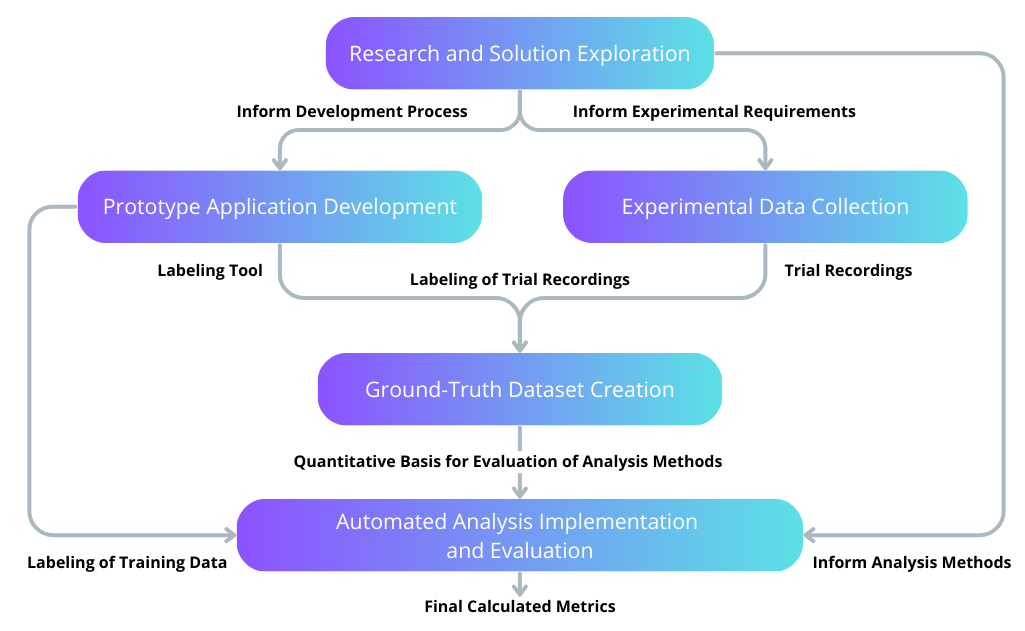
\includegraphics[width=0.8\textwidth]{methodology.png}
  \caption{Overview of the project phases, their deliverables, and the relationships between them.}
  \label{fig:methodology}
\end{figure*}

\paragraph{Research and Solution Exploration\\}
This initial phase aims to understand existing eyetracking analysis methods, 
relevant computer vision techniques, and to identify different solution strategies. 
The key deliverable of this phase is a documented analysis of state-of-the-art techniques and a selected solution strategy 
that will inform the experimental setup and automated analysis methods.

\paragraph{Prototype Application Development\\}
The objective is to develop a functional prototype application for annotating objects within the Care-lab simulation environments.
This tool will enable trainers to import eyetracking recordings, define simulation rooms and objects, and annotate them, 
serving as a foundation for ground-truth dataset creation.

\paragraph{Experimental Data Collection\\}
This phase focuses on gathering high-quality data from the Care-lab under controlled conditions. 
Students will be asked to observe medical domain-specific objects in the environment where the nature of the objects, 
the distance of the objects from the eye tracker, and the effect of varying backgrounds on detection accuracy are controlled for.
The deliverables are a set of eyetracking recordings and recordings of the objects in the environment.

\paragraph{Ground-Truth Dataset Creation\\}
The aim here is to create an accurate, frame-by-frame annotated ground-truth dataset from the experimental recordings. 
The developed prototype labeling tool will be used for manual annotation of observed objects, 
yielding a validated ground-truth dataset with observed objects for each frame.

\paragraph{Automated Analysis Implementation and Evaluation\\}
This final phase involves implementing and rigorously evaluating the selected automated analysis pipelines 
against the ground-truth dataset.
Activities include implementing various\\ approaches for object detection, segmentation, and image embedding, and quantitatively\\
assessing their performance (precision, recall, F1-score, ...).
The deliverables are a comparative performance analysis of these methods, demonstrating automated analysis capabilities.

\subsection{Timeline}

The project is planned to be completed between February 9, 2026 and May 30, 2026, with a total of 8 sprints of 2 weeks each.
Given that the internship was already completed in the first semester, three full days of work per week are set aside for the thesis.
The work will be split up into 8 sprints of two weeks each, with the first 7 sprints dedicated to the phases described above.
The final sprint (Sprint 8) is reserved as a buffer for any unforeseen delays or additional tasks that may arise during the project.

\section{Expected Results}
\label{sec:expected-results}

Based on the proposed methodology and the current state-of-the-art in computer vision, several outcomes are anticipated from this research.
The primary expectation is the successful development of a functional PoC software application. 
This application will demonstrate the feasibility of integrating computer vision models for automated analysis of observational performance in healthcare simulations.

Regarding the performance of the automated analysis methods, it is hypothesized that object detection models (e.g., fine-tuned YOLO variants or DINO) will yield the most robust and accurate results on the evaluation dataset.
This expectation stems from their inherent design to both localize and classify specific object categories for which they have been trained.

While open-set recognition models like\\ Grounding DINO, or classification approaches\\ based on image embeddings, offer flexibility by not requiring explicit retraining for every new object, they are anticipated to face challenges in this context.\\
The simulated environments contain a multitude of objects, many of which will be \textit{unknown} or irrelevant to the specific set of target objects for a given simulation.
This characteristic of the problem may lead to a higher number of false positives for pure classification models, a known challenge in open-set recognition tasks where the system must distinguish between known classes and a wide array of unseen distractors.
Object detection models, particularly if provided with sufficient training examples of the critical objects, are expected to be more discriminative and less prone to misclassification or false positives.

It is further expected that the system will be able to quantify gaze duration on identified objects with reasonable accuracy.
However, the degree of accuracy is contingent on both the resolution of the eyetracking recordings, and the quality of the provided gaze data.
Thus, it is expected that the system will struggle to accurately detect objects that are far away or not clearly visible in the eyetracking recordings. 

\section{Discussion, Expected\\ Conclusion}
\label{sec:discussion-conclusion}

The primary contribution of this research is a demonstration of the feasibility of 
integrating computer vision models with eyetracking data to objectively analyze performance in healthcare simulations.
While the PoC itself will be a prototype and not a production-ready application with comprehensive visualization dashboards, 
it will provide a solid foundation for future iterations and enhancements.
The instructors at HOGENT's 360° Care-lab will benefit from the clear indication that automated, 
objective assessment methods are achievable.

As computer vision is a rapidly developing\\ field, it is also anticipated that future advancements, 
particularly the continued rise of large foundation models, may enable even more sophisticated analysis methods. 
These could potentially allow for the analysis of eyetracking recordings with reduced reliance on extensive, 
domain-specific training datasets, though current computational costs for such large models can be a limiting factor. 
This research, therefore, not only addresses a current need but also positions the Care-lab to leverage future technological\\ progress in this domain.

\begingroup
\setlength{\emergencystretch}{3em}
\printbibliography[heading=bibintoc]
\endgroup

\end{document}